\documentclass[10pt,aspectratio=169]{beamer}

\usepackage{packages}
\usepackage{config}
\usepackage{appendixnumberbeamer}
\usetikzlibrary{decorations.pathmorphing,arrows.meta,positioning,calc,shapes.misc}

\graphicspath{ {./images/} }

\title[Un motor de un solo qubit]{Un motor de un solo qubit}
\subtitle{Termodinámica de un sistema de dos niveles}
\author{Hugo Campos}
\institute[USM]{Universidad Técnica Federico Santa María\\[2pt]\small Termodinámica y Mecánica Estadística}
\date{Noviembre de 2026}
\titlegraphic{
\includegraphics[width=1.5cm]{Logo_UTFSM.png}}

\setbeamertemplate{navigation symbols}{}
\setlength{\parskip}{4pt}
\newcommand{\grande}[1]{{\Large #1}}
\newcommand{\nota}[1]{{\small\color{gray}#1}}
\newcommand{\clave}[1]{{\color{usmBlue}\bfseries #1}}
\tikzset{
  foton/.style={decorate, decoration={snake, amplitude=1.6pt, segment length=5pt, post length=4pt}, -{Stealth[length=5pt]}, thick},
  nivel/.style={line width=1.6pt},
}
% un qubit dibujado: #1 = x, #2 = altura del nivel superior, #3 = 1 si está arriba
\newcommand{\qubit}[3]{%
  \draw[nivel, usmBlue] (#1-0.55,0) -- (#1+0.55,0);
  \draw[nivel, usmRed] (#1-0.55,#2) -- (#1+0.55,#2);
  \ifnum#3=1 \fill[usmYellow] (#1,#2) circle (4.5pt); \else \fill[usmYellow] (#1,0) circle (4.5pt); \fi
}

\begin{document}

%----------------------------------------------------------------- 1
\frame{\titlepage}

%----------------------------------------------------------------- 2
\begin{frame}{¿Puede un solo qubit ser un motor?}
\begin{columns}[c]
\begin{column}{0.48\textwidth}
  Un motor de auto tiene $\sim10^{23}$ moléculas: todo se promedia.

  \vspace{0.6em}
  Aquí la sustancia de trabajo es \clave{un sistema de dos niveles}: un qubit superconductor.

  \vspace{1em}
  Tres preguntas:
  \begin{enumerate}
  \setlength{\itemsep}{4pt}
  \item ¿Qué son el \clave{calor} y el \clave{trabajo} para un qubit?
  \item ¿Se cumplen las leyes de la termodinámica?
  \item ¿Qué cambia cuando el motor es tan pequeño?
  \end{enumerate}
\end{column}
\begin{column}{0.46\textwidth}\centering
  \begin{tikzpicture}[scale=0.9]
    % pistón
    \draw[thick] (0,0) rectangle (2.2,2.6);
    \fill[gray!25] (0.05,1.6) rectangle (2.15,1.85);
    \draw[thick] (1.1,1.85) -- (1.1,3.2);
    \foreach \x/\y in {0.4/0.4,1.0/0.9,1.6/0.5,0.6/1.2,1.8/1.2,1.3/0.3,0.3/0.8,1.5/1.0}
      \fill[usmBlue!60] (\x,\y) circle (2.5pt);
    \node[below] at (1.1,-0.15) {\small gas + pistón};
    % flecha
    \draw[-{Stealth[length=7pt]}, thick, gray] (2.7,1.3) -- (3.5,1.3);
    % qubit
    \begin{scope}[shift={(4.6,0.4)}]
      \qubit{0.6}{1.8}{1}
      \draw[<->, thick] (-0.2,0.1) -- node[left] {\small $\omega$} (-0.2,1.7);
      \node[below] at (0.6,-0.55) {\small un qubit};
    \end{scope}
  \end{tikzpicture}
\end{column}
\end{columns}
\end{frame}

%----------------------------------------------------------------- 3
\begin{frame}{Un qubit en contacto con un baño}
\begin{columns}[c]
\begin{column}{0.4\textwidth}\centering
  \begin{tikzpicture}[>=stealth]
    \draw[very thick, usmRed] (0,2) -- (2.6,2) node[right] {\small arriba: $\omega$};
    \draw[very thick, usmBlue] (0,0) -- (2.6,0) node[right] {\small abajo: $0$};
    \fill[usmYellow] (1.8,2) circle (5pt);
    \draw[<->, thick] (0.6,0.12) -- node[left] {\small brecha $\omega$} (0.6,1.88);
  \end{tikzpicture}

  \vspace{1.2em}
  Probabilidad de estar arriba (Gibbs):
  \[ p_{\mathrm{eq}} = \frac{1}{1 + e^{\omega/T}} \]
  \nota{la brecha $\omega$ se controla desde afuera con un flujo magnético}
\end{column}
\begin{column}{0.56\textwidth}\centering
  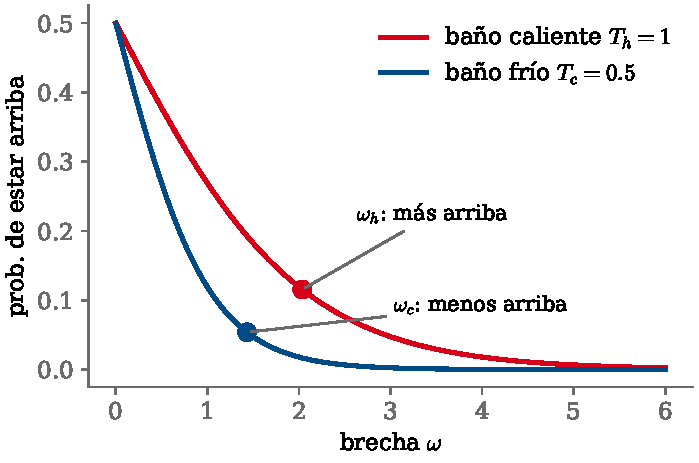
\includegraphics[width=\linewidth]{s_poblacion.pdf}
\end{column}
\end{columns}
\end{frame}

%----------------------------------------------------------------- 4
\begin{frame}{Primera ley a escala de un qubit}
\begin{center}
\renewcommand{\arraystretch}{1.5}
\begin{tabular}{lccccc}
 & & & \textcolor{gray}{\small calor recibido} & & \textcolor{gray}{\small trabajo recibido}\\
\textbf{Gas:} & $\mathrm{d}U$ & $=$ & $T\,\mathrm{d}S$ & $+$ & $(-P\,\mathrm{d}V)$\\
\textbf{Qubit} \small($E=\omega p$): & {\Large$\mathrm{d}E$} & {\Large$=$} & {\Large$\omega\,\mathrm{d}p$} & {\Large$+$} & {\Large$p\,\mathrm{d}\omega$}
\end{tabular}
\end{center}
\vspace{0.1em}
\begin{columns}[t]
\begin{column}{0.46\textwidth}\centering
  \begin{tikzpicture}
    \qubit{0}{1.6}{0}
    \draw[->, thick, gray] (0.9,0.8) -- (1.5,0.8);
    \qubit{2.4}{1.6}{1}
    \draw[foton, usmRed] (3.6,2.3) -- (2.75,1.75);
  \end{tikzpicture}

  \vspace{0.4em}
  \clave{Calor:} los niveles quietos,\\ cambia la probabilidad.\\
  \nota{el qubit absorbe o emite un fotón del baño}
\end{column}
\begin{column}{0.46\textwidth}\centering
  \begin{tikzpicture}
    \qubit{0}{1.9}{1}
    \draw[->, thick, gray] (0.9,0.8) -- (1.5,0.8);
    \qubit{2.4}{1.1}{1}
    \draw[dashed, gray] (1.85,1.9) -- (2.95,1.9);
    \draw[->, thick, usmGreen] (3.15,1.9) -- (3.15,1.15);
  \end{tikzpicture}

  \vspace{0.4em}
  \clave{Trabajo:} la probabilidad quieta,\\ se mueve el nivel.\\
  \nota{la energía va al campo que controla la brecha}
\end{column}
\end{columns}
\end{frame}

%----------------------------------------------------------------- 5
\begin{frame}{Diccionario: gas en un cilindro $\leftrightarrow$ qubit}
\begin{columns}[c]
\begin{column}{0.62\textwidth}
\renewcommand{\arraystretch}{1.35}
\begin{tabular}{ll}
\toprule
\textbf{Gas} & \textbf{Qubit}\\
\midrule
volumen $V$ & brecha $\omega$\\
presión $P$ & población excitada $p$\\
trabajo $P\,\mathrm{d}V$ & trabajo $p\,\mathrm{d}\omega$\\
calor $T\,\mathrm{d}S$ & calor $\omega\,\mathrm{d}p$\\
pistón & campo magnético que fija $\omega$\\
isocora ($V$ fijo) & contacto con un baño a $\omega$ fijo\\
adiabática ($S$ fija) & cambiar $\omega$ con $p$ fija\\
expandirse entrega trabajo & \clave{achicar la brecha} entrega trabajo\\
\bottomrule
\end{tabular}
\end{column}
\begin{column}{0.34\textwidth}
  ¿Por qué $p$ fija es adiabática?

  \vspace{0.3em}
  La entropía del qubit depende solo de $p$:
  \[ S = -p\ln p - (1-p)\ln(1-p) \]
  Si $p$ no cambia, $S$ no cambia.

  \vspace{0.6em}
  \nota{Ojo con el signo: en el gas el trabajo sale al crecer $V$; en el qubit, al bajar $\omega$.}
\end{column}
\end{columns}
\end{frame}

%----------------------------------------------------------------- 6
\begin{frame}{El ciclo de Otto, fotón por fotón}
\begin{center}
\begin{tikzpicture}[x=1cm,y=1cm]
  % 1
  \qubit{0}{2.2}{1}
  \draw[foton, usmRed] (-1.3,3.0) -- (-0.3,2.35);
  \node[usmRed] at (-1.3,3.25) {\small $\omega_h$};
  \node at (0,-0.6) {\small \textbf{1.} baño caliente};
  \node at (0,-1.0) {\small absorbe $\omega_h$};
  % 2
  \qubit{3.6}{1.3}{1}
  \draw[dashed, gray] (3.05,2.2) -- (4.15,2.2);
  \draw[->, thick, usmGreen] (4.4,2.2) -- (4.4,1.35);
  \node[usmGreen, right] at (4.45,1.8) {\small $\omega_h-\omega_c$};
  \node at (3.6,-0.6) {\small \textbf{2.} se achica la brecha};
  \node at (3.6,-1.0) {\small \textcolor{usmGreen}{trabajo entregado}};
  % 3
  \qubit{7.4}{1.3}{0}
  \draw[foton, usmBlue] (7.7,1.25) -- (8.7,1.95);
  \node[usmBlue] at (8.9,2.15) {\small $\omega_c$};
  \node at (7.4,-0.6) {\small \textbf{3.} baño frío};
  \node at (7.4,-1.0) {\small emite $\omega_c$};
  % 4
  \qubit{11}{2.2}{0}
  \draw[dashed, gray] (10.45,1.3) -- (11.55,1.3);
  \draw[->, thick, gray] (11.8,1.35) -- (11.8,2.15);
  \node at (11,-0.6) {\small \textbf{4.} se agranda la brecha};
  \node at (11,-1.0) {\small gratis (está abajo)};
  % flechas entre etapas
  \foreach \x in {1.5,5.3,9.1} \draw[-{Stealth[length=6pt]}, thick, gray!70] (\x,1.1) -- (\x+0.7,1.1);
\end{tikzpicture}
\end{center}
\vspace{0.4em}
\begin{center}
\renewcommand{\arraystretch}{1.3}
\begin{tabular}{ccccc}
entra del baño caliente & & sale como trabajo & & va al baño frío\\
$Q_h = \omega_h$ & $=$ & $W = \omega_h - \omega_c$ & $+$ & $Q_c = \omega_c$
\end{tabular}

\vspace{0.4em}
\nota{Si en el paso 4 el qubit sigue arriba, hay que pagar $\omega_h-\omega_c$: por eso el trabajo fluctúa.}
\end{center}
\end{frame}

%----------------------------------------------------------------- 7
\begin{frame}{¿Cómo se construye y quién recibe el trabajo?}
\begin{columns}[c]
\begin{column}{0.58\textwidth}\centering
\begin{tikzpicture}[scale=0.95, every node/.style={font=\small}]
  % qubit (lazo con dos uniones)
  \draw[very thick] (-0.7,-0.6) rectangle (0.7,0.6);
  \foreach \y in {-0.6,0.6} \node[cross out, draw, thick, minimum size=7pt, inner sep=0pt, fill=white] at (0,\y) {};
  \node at (0,0) {qubit};
  % bobina de flujo
  \draw[thick, usmGreen] (-0.5,1.4) -- (0.5,1.4);
  \foreach \x in {-0.4,-0.1,0.2} \draw[thick, usmGreen] (\x,1.4) arc (180:0:0.15);
  \draw[-{Stealth}, thick, usmGreen] (0,2.4) -- (0,1.75);
  \node[usmGreen, align=center] at (0,2.85) {flujo $\Phi(t)$: fija la brecha\\ \textbf{recibe el trabajo}};
  % resonador caliente
  \draw[thick, usmRed] (-1.6,0) -- (-0.7,0);
  \draw[thick, usmRed, rounded corners] (-3.6,-1) rectangle (-1.6,1);
  \node[usmRed, align=center] at (-2.6,0.35) {LC a $\omega_h$};
  \node[usmRed, align=center] at (-2.6,-0.35) {$R_H$ a $T_h$};
  \node[usmRed] at (-2.6,-1.35) {baño caliente};
  % resonador frío
  \draw[thick, usmBlue] (0.7,0) -- (1.6,0);
  \draw[thick, usmBlue, rounded corners] (1.6,-1) rectangle (3.6,1);
  \node[usmBlue] at (2.6,0.35) {LC a $\omega_c$};
  \node[usmBlue] at (2.6,-0.35) {$R_C$ a $T_c$};
  \node[usmBlue] at (2.6,-1.35) {baño frío};
\end{tikzpicture}

\vspace{0.6em}
{\small\raggedright
\textbf{LC:} circuito resonante (bobina $L$ + condensador $C$). Solo intercambia energía a su frecuencia, como un filtro.\\[2pt]
\textbf{R:} resistencia a temperatura $T$. Sus electrones en agitación térmica son el baño.
}
\end{column}
\begin{column}{0.38\textwidth}
  Los baños \clave{se abren y cierran por resonancia}:
  \begin{itemize}
  \item brecha $=\omega_h$: intercambia calor con $R_H$;
  \item brecha $=\omega_c$: intercambia calor con $R_C$;
  \item en medio: aislado.
  \end{itemize}

  \vspace{0.4em}
  El flujo externo es el \clave{pistón y el cigüeñal}: mueve la brecha y recibe el trabajo, que es electromagnético.

  \vspace{0.4em}
  \nota{Propuesta de Karimi y Pekola (2016), como refrigerador; al revés, es un motor.}
\end{column}
\end{columns}
\end{frame}

%----------------------------------------------------------------- 8
\begin{frame}{Eficiencia: la segunda ley aparece sola}
\begin{columns}[c]
\begin{column}{0.46\textwidth}\centering
  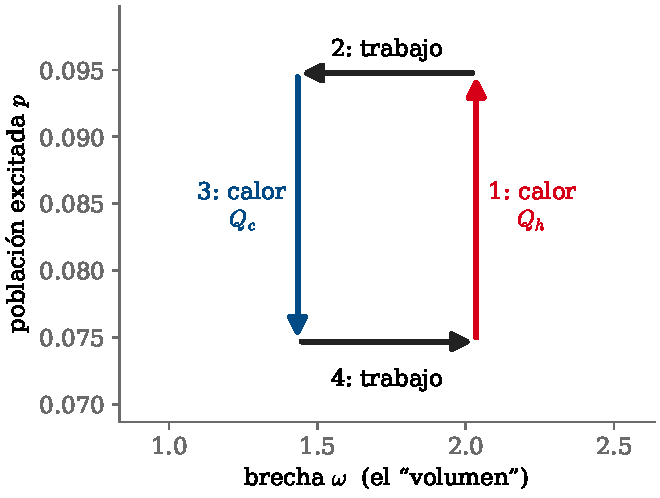
\includegraphics[width=\linewidth]{s_ciclo.pdf}\\
  \nota{en promedio: el área encerrada es el trabajo}
\end{column}
\begin{column}{0.5\textwidth}
  \[ \eta = \frac{W}{Q_h} = 1 - \frac{\omega_c}{\omega_h} \]

  Para que sea motor, el baño caliente debe dejar \clave{más} población arriba que el frío:
  \[
  \frac{1}{1+e^{\omega_h/T_h}} > \frac{1}{1+e^{\omega_c/T_c}}
  \;\Longleftrightarrow\;
  \frac{\omega_c}{\omega_h} > \frac{T_c}{T_h}
  \]
  \[ \Longrightarrow \quad \eta < 1 - \frac{T_c}{T_h} = \eta_C \]
  \nota{Nadie impuso Carnot: sale de la estadística de Gibbs.}
\end{column}
\end{columns}
\end{frame}

%----------------------------------------------------------------- 9
\begin{frame}{Tiempo finito: potencia contra eficiencia}
\begin{center}
  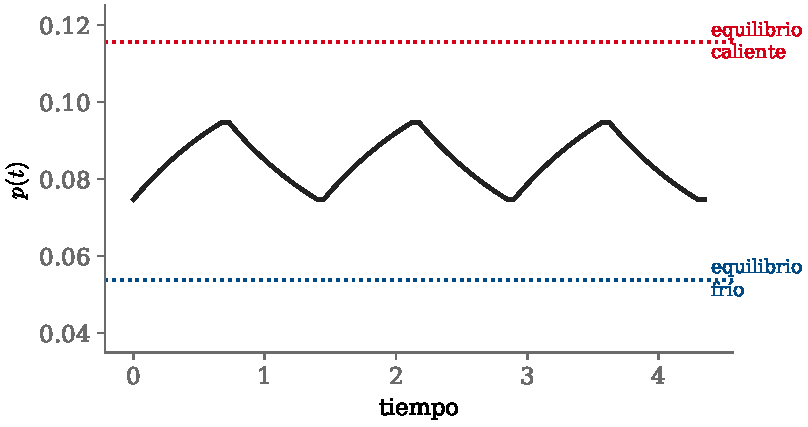
\includegraphics[width=0.62\linewidth]{s_pt.pdf}
\end{center}
\begin{columns}[t]
\begin{column}{0.45\textwidth}
  \clave{Contactos cortos:} no alcanza a pasar calor.\\
  \clave{Contactos largos:} la potencia se va a cero.
\end{column}
\begin{column}{0.45\textwidth}
  A potencia máxima: $\eta = 0{,}296$\\
  Curzon--Ahlborn: $1-\sqrt{T_c/T_h} = 0{,}293$
\end{column}
\end{columns}
\end{frame}

%----------------------------------------------------------------- 10
\begin{frame}{Lo nuevo a esta escala: el motor fluctúa}
\begin{columns}[c]
\begin{column}{0.54\textwidth}\centering
  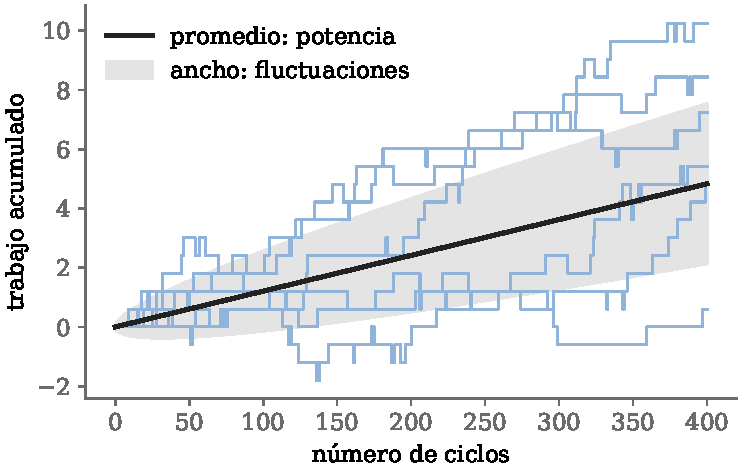
\includegraphics[width=\linewidth]{s_trayectorias.pdf}
\end{column}
\begin{column}{0.42\textwidth}
  Cada ciclo el qubit está \clave{arriba o abajo}: el trabajo es aleatorio.

  \vspace{0.6em}
  Relación de incertidumbre termodinámica:
  \[ \Delta P \cdot \Sigma \;\ge\; 2P^2 \]
  \nota{fluctuaciones $\times$ entropía producida $\ge$ 2 $\times$ potencia$^2$}

  \vspace{0.4em}
  \grande{La precisión \clave{cuesta disipación}.}

  \vspace{0.4em}
  Los mejores ciclos están justo en el límite.
\end{column}
\end{columns}
\end{frame}

%----------------------------------------------------------------- 11
\begin{frame}{\emph{Fun fact}: optimizar el motor}
\begin{center}
  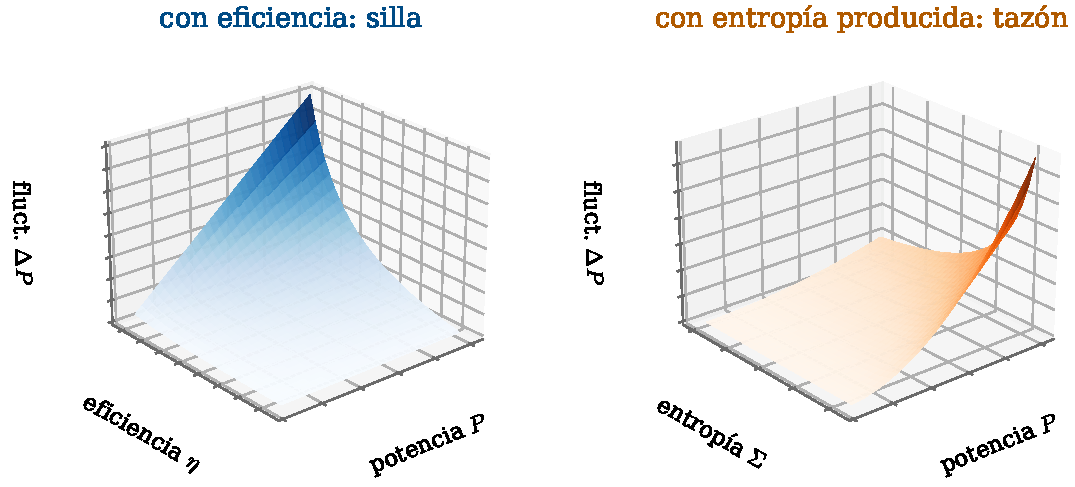
\includegraphics[height=0.53\textheight]{s_silla.pdf}
\end{center}
\vspace{-0.4em}
\begin{columns}[t]
\begin{column}{0.46\textwidth}\centering
  Con \clave{eficiencia}: \clave{silla}.\\
  Una figura de mérito $aP + b\eta - c\,\Delta P$ encuentra solo el 11\%.
\end{column}
\begin{column}{0.46\textwidth}\centering
  Con \clave{entropía}: \clave{canaleta convexa}.\\
  La misma figura de mérito los encuentra todos.
\end{column}
\end{columns}
\vspace{0.2em}
\begin{center}
\nota{Misma idea que la construcción de Maxwell. Los ciclos los encontramos con algoritmos evolutivos multiobjetivo.}
\end{center}
\end{frame}

%----------------------------------------------------------------- 12
\begin{frame}{Conclusiones}
\vspace{0.6em}
\begin{enumerate}
\setlength{\itemsep}{1.2em}
\item[\color{usmBlue}\Large 1] \grande{Un qubit es un motor térmico completo.}\\
  Calor: cambiar probabilidades. Trabajo: mover los niveles. El campo de control es el pistón.
\item[\color{usmBlue}\Large 2] \grande{La termodinámica clásica aparece sola.}\\
  Carnot sale de Gibbs; a potencia máxima, Curzon--Ahlborn.
\item[\color{usmBlue}\Large 3] \grande{Lo nuevo es que fluctúa.}\\
  La precisión cuesta disipación, y los mejores ciclos están en ese límite.
\end{enumerate}
\end{frame}

%----------------------------------------------------------------- cierre
{
\setbeamercolor{background canvas}{bg=usmBlue}
\setbeamertemplate{footline}{}
\begin{frame}[plain]
  \vfill
  \begin{center}
    {\color{white}\Huge ¡Gracias!}\\[10pt]
    {\color{white}\large ¿Preguntas?}
  \end{center}
  \vfill
\end{frame}
}

%================================================================= respaldo
\appendix

\begin{frame}{Respaldo 1: la entropía del qubit}
\begin{columns}[c]
\begin{column}{0.52\textwidth}\centering
  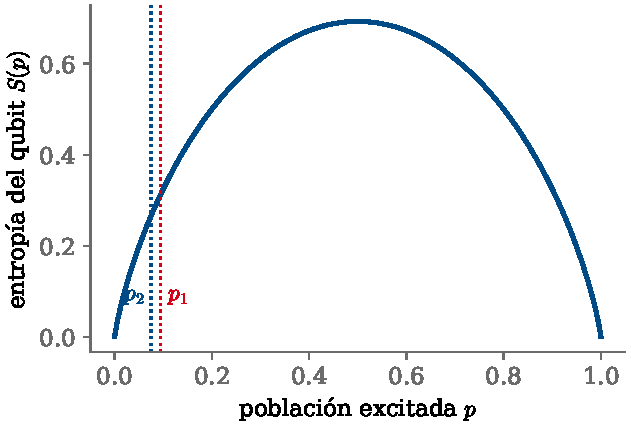
\includegraphics[width=\linewidth]{s_entropia.pdf}
\end{column}
\begin{column}{0.44\textwidth}
  \[ S(p) = -p\ln p - (1-p)\ln(1-p) \]
  \begin{itemize}
  \item Solo depende de $p$: cambiar $\omega$ con $p$ fija es \clave{isentrópico}.
  \item En los baños, $p$ oscila entre $p_2$ y $p_1$: la entropía del qubit vuelve a su valor en cada ciclo.
  \item Toda la entropía producida termina en los baños:
  \[ \Sigma = \frac{Q_c}{T_c} - \frac{Q_h}{T_h} \ge 0 \]
  \end{itemize}
\end{column}
\end{columns}
\end{frame}

\begin{frame}{Respaldo 2: cómo se calculan las fluctuaciones}
Cada ciclo es una cadena de Markov. Se pesa cada salto por $e^{\chi w}$:
\[
\mathcal{T}(\chi)_{ss'} = \sum_{s_1} M^h_{s s_1}\, e^{\chi\Delta\omega s_1}\, M^c_{s_1 s'}\, e^{-\chi\Delta\omega s'},
\qquad
\theta(\chi) = \ln \lambda_{\max}\bigl(\mathcal{T}(\chi)\bigr)
\]
\vspace{0.3em}
\[
P = \frac{\theta'(0)}{\tau_{\text{ciclo}}}, \qquad \Delta P = \frac{\theta''(0)}{\tau_{\text{ciclo}}}
\]
\begin{itemize}
\item $\theta$ es el ``$\ln Z$'' del trabajo: derivarla da los cumulantes, con las correlaciones entre ciclos incluidas.
\item $\det\mathcal{T}$ no depende de $\chi$, así que todo sale en forma cerrada.
\item Validado con simulación Monte Carlo.
\end{itemize}
\end{frame}

\begin{frame}{Respaldo 3: los algoritmos (30 semillas)}
\begin{center}
  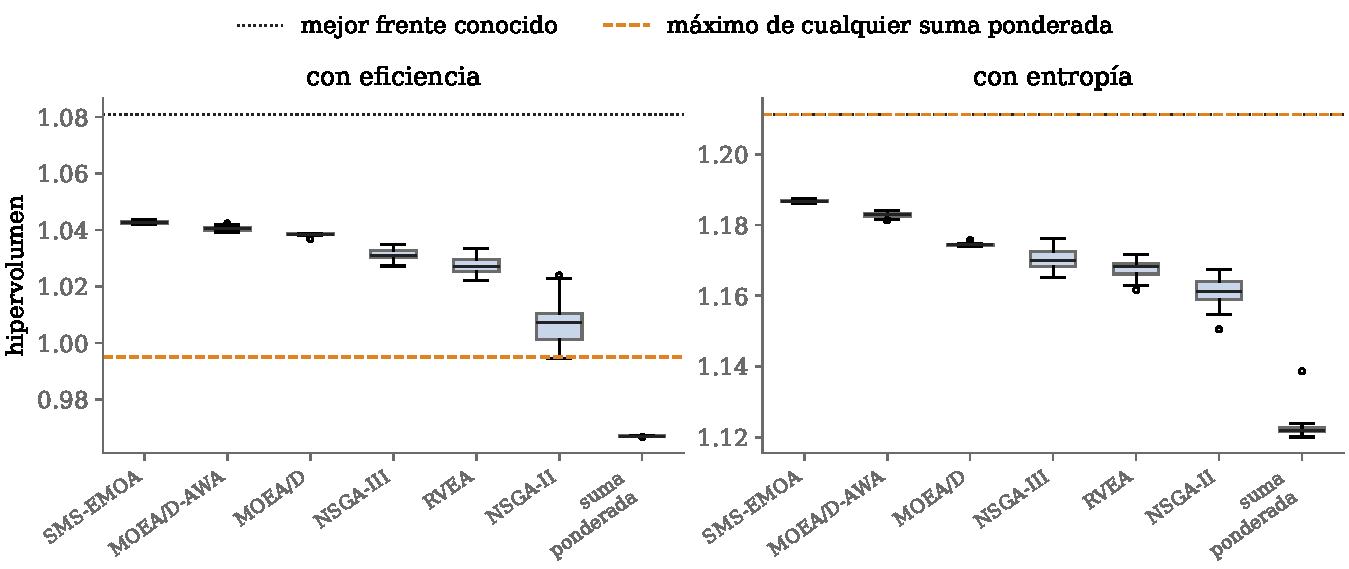
\includegraphics[width=0.92\linewidth]{s_hv_otto.pdf}
\end{center}
\begin{center}
Con $\eta$, \clave{6 de 7 algoritmos superan el máximo de cualquier suma ponderada}.
\end{center}
\end{frame}

\begin{frame}{Respaldo 4: cerca del equilibrio}
\begin{columns}[c]
\begin{column}{0.52\textwidth}\centering
  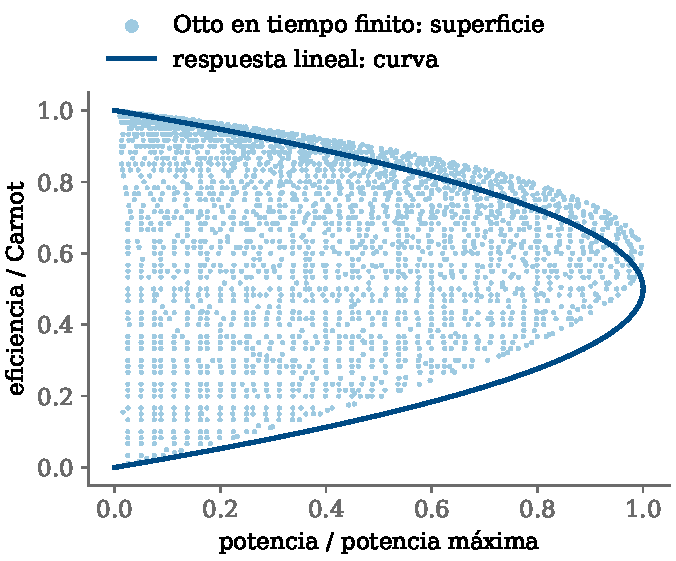
\includegraphics[width=\linewidth]{s_lr.pdf}
\end{column}
\begin{column}{0.44\textwidth}
  En respuesta lineal (Onsager), con acoplamiento fuerte, todo depende de \clave{un solo número} $e$:
  \[ P = e(1-e),\quad \bar\eta = e,\quad \Sigma = (1-e)^2 \]
  Potencia y eficiencia van amarradas: el frente es una \clave{curva}.

  \vspace{0.5em}
  \nota{Almanza-Marrero, Roldán y Manzano (2026). Lejos del equilibrio se desacoplan.}
\end{column}
\end{columns}
\end{frame}

\begin{frame}{Referencias}
\small
\begin{itemize}
\setlength{\itemsep}{4pt}
\item B. Karimi y J.\,P. Pekola, \emph{Otto refrigerator based on a superconducting qubit: classical and quantum performance}, arXiv:1610.02776 (2016).
\item P. Pietzonka y U. Seifert, \emph{Phys. Rev. Lett.} \textbf{120}, 190602 (2018).
\item P.\,A. Erdman \emph{et al.}, \emph{Phys. Rev. Research} \textbf{5}, L022017 (2023).
\item F.\,L. Curzon y B. Ahlborn, \emph{Am. J. Phys.} \textbf{43}, 22 (1975).
\item J.\,A. Almanza-Marrero, É. Roldán y G. Manzano, arXiv:2603.19885 (2026).
\end{itemize}
\end{frame}

\end{document}
